% `template.tex', a bare-bones example employing the AIAA class.
%
% For a more advanced example that makes use of several third-party
% LaTeX packages, see `advanced_example.tex', but please read the
% Known Problems section of the users manual first.
%
% Typical processing for PostScript (PS) output:
%
%  latex template
%  latex template   (repeat as needed to resolve references)
%
%  xdvi template    (onscreen draft display)
%  dvips template   (postscript)
%  gv template.ps   (onscreen display)
%  lpr template.ps  (hardcopy)
%
% With the above, only Encapsulated PostScript (EPS) images can be used.
%
% Typical processing for Portable Document Format (PDF) output:
%
%  pdflatex template
%  pdflatex template      (repeat as needed to resolve references)
%
%  acroread template.pdf  (onscreen display)
%
% If you have EPS figures, you will need to use the epstopdf script
% to convert them to PDF because PDF is a limmited subset of EPS.
% pdflatex accepts a variety of other image formats such as JPG, TIF,
% PNG, and so forth -- check the documentation for your version.
%
% If you do *not* specify suffixes when using the graphicx package's
% \includegraphics command, latex and pdflatex will automatically select
% the appropriate figure format from those available.  This allows you
% to produce PS and PDF output from the same LaTeX source file.
%
% To generate a large format (e.g., 11"x17") PostScript copy for editing
% purposes, use
%
%  dvips -x 1467 -O -0.65in,0.85in -t tabloid template
%
% For further details and support, read the Users Manual, aiaa.pdf.


% Try to reduce the number of latex support calls from people who
% don't read the included documentation.
%
\typeout{}\typeout{If latex fails to find aiaa-tc, read the README file!}
%


\documentclass[]{aiaa-tc}% insert '[draft]' option to show overfull boxes
\usepackage{amsmath}								%For mathematical typesetting
\usepackage{amssymb}								%For mathematical typesetting

 \title{A High-order Conservative Eulerian Simulation Method for Vortex Dominated Flows}

 \author{
 Joshua J. Bevan%
    \thanks{Graduate Student, University of Massachusetts Lowell, Lowell, Massachusetts 01854.}\\
  {\normalsize\itshape
   University of Massachusetts Lowell, Lowell, Massachusetts, 01854, USA}\\
 }

 % Data used by 'handcarry' option if invoked
 \AIAApapernumber{YEAR-NUMBER}
 \AIAAconference{Conference Name, Date, and Location}
 \AIAAcopyright{\AIAAcopyrightD{YEAR}}

 % Define commands to assure consistent treatment throughout document
 \newcommand{\eqnref}[1]{(\ref{#1})}
 \newcommand{\class}[1]{\texttt{#1}}
 \newcommand{\package}[1]{\texttt{#1}}
 \newcommand{\file}[1]{\texttt{#1}}
 \newcommand{\BibTeX}{\textsc{Bib}\TeX}

\newcommand{\be}{\begin{equation}}
\newcommand{\ben}[1]{\begin{equation}\label{#1}}
\newcommand{\ee}{\end{equation}}
\newcommand{\aomega}{\overset{\sim}{\omega}}				%Approximate omega

\begin{document}

\maketitle

%============================================================
\begin{abstract}
A high-order, conservative Eulerian method is presented for the simulation of vortex dominated inviscid fluid flows. The primitive variable incompressible Euler equations are recast in the velocity-vorticity form to explicitly enforce conservation of vorticity. The advection of the vorticity is then calculated via a two-step process: the velocity field is determined by evaluation of the Biot-Savart integral, and then a line-based discontinuous Galerkin (DG) Eulerian spatial discretization scheme is applied to accurately advect the vorticity field. The accuracy and convergence of this method was examined for test cases where an analytical solution exists, as well as more challenging test cases which lack an analytical solution. The convergence rate behavior is chiefly controlled by the error in the calculated velocity field. Velocity errors are due to two factors: the approximation of the Biot-Savart integral with a desingularized form, and poor quadrature convergence for the nearly singular integral. Solver parameters were chosen to balance these two effects resulting in nearly optimal convergence of the overall method in the analytical test, and high-order convergence in the qualitative test case.
\end{abstract}

%============================================================
\section*{Nomenclature}

%\begin{tabbing}
%  XXX \= \kill% this line sets tab stop
%  $J$ \> Jacobian Matrix \\
%  $f$ \> Residual value vector \\
%  $x$ \> Variable value vector \\
%  $F$ \> Force, N \\
%  $m$ \> Mass, kg \\
%  $\Delta x$ \> Variable displacement vector \\
%  $\alpha$ \> Acceleration, m/s\textsuperscript{2} \\[5pt]
%  \textit{Subscript}\\
%  $i$ \> Variable number \\
% \end{tabbing}

%============================================================
\section{Introduction}
Direct solution of Navier-Stokes is impractical for many fluid problems and where possible simplifications should be made; one such possibility is for vortex dominated flows. It is possible to recast Navier-Stokes from a primitive variable form ($u,v,p$) to a velocity-vorticity ($u,v,\omega$) form. This has several advantages: explicit conservation of vorticity, elimination of pressure terms (for incompressible flows), and reduction of required simulated degrees of freedom to just those that form the vorticity support.

Many vortex based simulation techniques use a Lagrangian approach to discretize the vorticity into a set of vortex particles\cite{Point4}, lines\cite{Line4}, sheets\cite{Sheet1}, or volumes\cite{Volume1}. This is a natural approach to take given the material nature of the vorticity due to Helmholtz and Kelvin's theorems.

%Lagrangian codes
The velocity field due to the vorticity is calculated from solving the Poisson problem \cite{MiscMeth1}, or through inversion of the Poisson problem via evaluation of the Biot-Savart integral \cite{Saffman1992}. There are several challenges with evaluation of the velocity: boundary conditions in the Poisson solution method, and singularities in the Biot-Savart volume integral method. Typically Lagrangian point vortex codes must de-singularize the kernel \cite{Rosenhead1930,Moore1972}. Direct summation for the velocity field has a $\mathcal{O}(N^2)$ complexity. Tree-codes \cite{LindsayKrasny2001} and Fast Multipole Methods (FMM) \cite{Strain1997} are ways of achieving a more efficient calculation.

Lagrangian point methods present several problems. Point disorganization can occur as the fluid evolves, this typically requires temporary meshing to recondition the discretization. This has been handled with various methods; recalculation of the quadrature weights at each time step \cite{Remesh2,Remesh3}, regridding/rezoning \cite{Remesh4}, and remeshing \cite{Remesh5} among them. Additionally, most Lagrangian approaches are limited to low order; careful point locations must be chosen and maintained through frequent remeshing etc. in order to achieve high-order convergence \cite{Strain1997}.

%Existing Eulerian codes
In comparison, Eulerian approaches to vortex methods tend to be less common. Work has been done for viscous flows with solid bodies; both stationary \cite{MiscMeth3} and moving \cite{MiscMeth2}. Both of these solve the streamfunction-vorticity formulation, not the velocity-vorticity formulation. The velocity-vorticity formulation has been solved by an Eulerian approach by others \cite{MiscMeth4}. A notable example of an Eulerian approach to the velocity-vorticity formulation is the work of Brown et al. \cite{Brown2000} who adapted the velocity-vorticity approach to a low order Finite Volume (FV) solver. Later they were able to extend their method to be accelerated via a FMM \cite{Brown2004}. However, like most FV approaches, to extend to high order solution approximations requires extended stencils that ultimately limit the geometrical freedom of the mesh. Steinhoff et al. also used an Eulerian approach, but solved a modified form of the inviscid Euler equations with ``vorticity confinement'' rather than the velocity-vorticity equation \cite{SteinhoffUnderhill1994}.

The desire to resolve fine vortical structures motivates the need for a high order solver. Considering the challenges associated with achieving a high order Lagrangian method and the success of Brown et al.'s low order method, a high order Eulerian vorticity-velocity method would seem to be a possible choice. This leaves the choice of a spatial discretization.

Finite difference methods suffer from similar problems as FV with extended stencils, as well as not being explicitly conservative. A finite element approach is ill-suited to the hyperbolic nature of vorticity advection. Spectral methods are promising, but for sparse vorticity domains are less-efficient due to the global support of the harmonic bases. However, discontinuous Galerkin (DG) methods \cite{HestWar} are a natural choice; they are conservative, able to take advantage of vorticity sparseness, are well-suited to handle advection via intelligent choice of a numerical flux function, and have bases with local/compact support.

For domains free of impinging bodies a hexahedral mesh with a tensor product grid of interpolation points is convenient to implement. This permits the use of a line-DG \cite{Persson2013} approach that considerably simplifies multi-dimensional cases by allowing reuse of 1D methods. Choosing a 2D domain permits evaluation of whether the method is practical, as well as to limit solution times to those that are reasonable on a workstation. It also has the advantage of removing the vortex stretching term and reducing the vorticity to a scalar. The resultant partial differential equation (PDE) takes on the familiar form of a scalar conservation law. To maintain maximum flexibility for investigative purposes and to remove as much approximation error as possible the velocity field for validation of the underlying method is calculated via direct evaluation of the Biot-Savart integral.

%============================================================
\section{Governing Equations and Spatial Discretization}

The Navier-Stokes momentum equation is
 \be \rho \left(\frac{\partial \mathbf{u}}{\partial t} + \mathbf{u} \cdot \nabla \mathbf{u} \right) = -\nabla p + \mu \nabla^2 \mathbf u + \tfrac13 \, \mu \nabla (\nabla\cdot\mathbf{u}) \ee
where $u$ is the velocity field, $p$ is the pressure, and $\rho$ is the density. If we restrict ourselves to incompressible flows and define the quantity \textit{vorticity} as
\be \mathbf{\omega} = \nabla \times \mathbf{u} \ee
Then the traditional form of the Navier-Stokes equations can be recast
\ben{VV3D} \frac{\partial \omega}{\partial t} +  \mathbf{u} \cdot \nabla \omega - \omega \cdot \nabla  \mathbf{u} = S(x,t)\ee
where we collect viscous generation of vorticity in $S$.

For 2-D distributions of vorticity, several simplifications can be made. The originally vectorial vorticity becomes a scalar quantity, all vorticity is directed normal to the plane. As a result, the vortex stretching term in  Eqn.\,\eqref{VV3D} becomes zero. The only non-zero component of $\omega$ is in the z-direction, however the gradient of the velocity field is zero in the z-direction, so the product is therefore zero. The result is
\ben{VV2D} \frac{\partial \omega}{\partial t} + u \cdot \nabla \omega = S(x,t)\ee
or if instead the second term is expressed in terms of the flux of the vorticity (where $f_i(\omega)=u_i\,\omega$):
\ben{VV2DB} \frac{\partial \omega}{\partial t} + \frac{\partial f}{\partial x_i}= S(x,t)\ee

 For an incompressible 2D or 3D flow we can relate the velocity and vorticity by:
\be \nabla^2 u = -\nabla \times \omega \ee
If inverted, the Biot-Savart integral is obtained
\ben{BS} u(x^*) = \int_\Omega K(x^*,x) \times \omega(x) dx \ee
where $x^*$ is the point we wish to evaluate the velocity, $x$ is the coordinate in regions of non-zero vorticity, and $K(x^*,x)$ is the singular Biot-Savart kernel \cite{BealeMajda}
\ben{BSkern} K(x^*,x) = \frac{-1}{2 \pi} \frac{x^*-x}{|x^*-x|^2} \ee

The high-order Eulerian approach taken here means that while the Biot-Savart integral converges, a singularity is always present within any of the extended vorticity patches thanks to self-influence. Conceptually this doesn't present an impossible problem, the integral \textit{does} converge in an analytical sense; practically speaking however a singularity may cause numerical integration procedures to diverge, or at the very least converge quite slowly. The approach taken by Brown \cite{Brown2004} was to use the Rosenhead-Moore kernel, choosing a core size such that the maximum velocity occurred on the face of the finite volume unit. This can be constructed \textit{a priori} because the vorticity is taken as constant across the volume, as is typical in a FV approach. If the vorticity is spatially varying however, the choice of core size is more troublesome.

One may attempt to desingularize the Biot-Savart kernel by introducing a core function $\eta(^z/_{\delta})$, with characteristic cutoff radius $\delta$. Traditionally the core function is convolved with the Biot-Savart kernel to yield a desingularized kernel $K_{\delta}$.
\ben{DesingBS} K*\eta(r) = K_{\delta} \ee

The choice of a core function and a characteristic radius has important implications on the accuracy and convergence of a Lagrangian point vortex method. Choosing a cutoff radius too small and there is insufficient smoothing, too large and the vorticity discretization is spatially smeared. In a Lagrangian method the convolution with a core function has a physical heuristic: the point vortex is replaced by a finite size vortex blob described by $\eta(r)$, with characteristic radius $\delta$. 

In the present method the core function is a means to an end; attempting to numerically integrate the singular Biot-Savart integral will result in spurious values, so the desingularized kernel is used as an approximation. A number of kernels can be chosen in a Lagrangian method, we found the following kernel\cite{WL} generally had the lowest approximation error:
\ben{PSkern0}  K_{spectral}= \frac{z}{2 \pi |z|^2} (1-J_0(\frac{z}{\delta})) \ee
where we have substituted $z=x^*-x$, and $J_\alpha$ are Bessel functions of the first kind. 

%============================================================
\section{Results}

In this section we will introduce some figures and tables.
It can be seen in figure~\ref{f:magnetic_field} that magnetization is a
function of applied field.
\begin{figure}[htb]% order of placement preference: here, top, bottom
 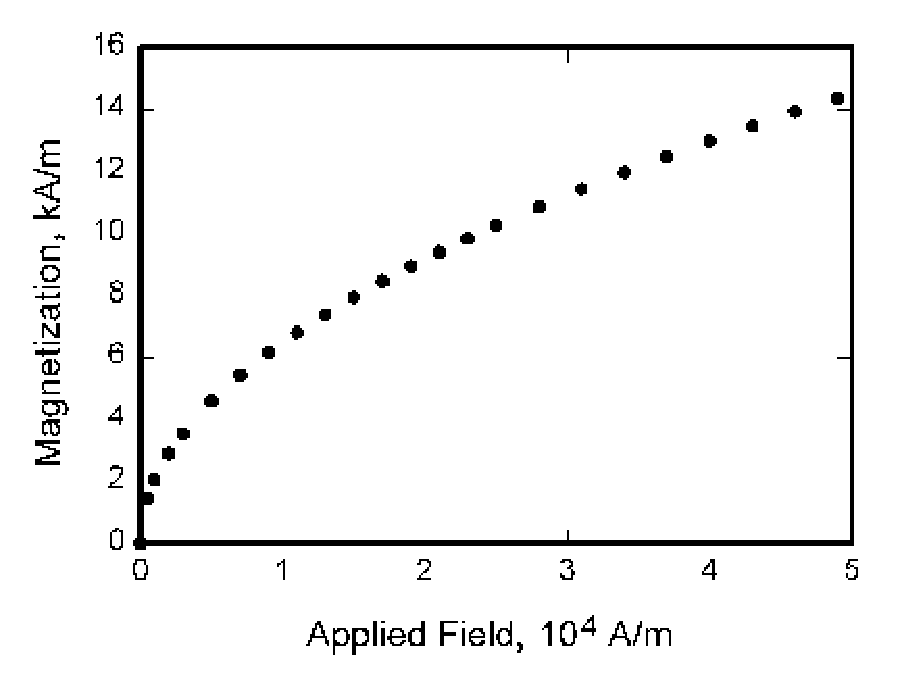
\includegraphics{figure_magnet}
 \caption{Magnetization as a function of applied field, which has
   borders so thick that they overwhelm the data and for some reason the
   ordinate label is rotated 90 degrees to make it difficult to
   read. This figure also demonstrates the dangers of using a bitmap
   as opposed to a vector image.}
 \label{f:magnetic_field}
\end{figure}
Sometimes writing meaningless text can be quiet easy, but other times
one is hard pressed to keep the words flowing.\footnote{And sometimes
things get carried away in endless detail.}
Meanwhile back in the other world, table~\ref{t:scheme_comparison} shows
a nifty comparison.
\begin{table}% no placement specified: defaults to here, top, bottom, page
 \begin{center}
  \caption{Variable and Fixed Coefficient Runge-Kutta Schemes as a
           Function of Reynolds Number}
  \label{t:scheme_comparison}
  \begin{tabular}{rrr}
       Re & Vary & Fixed \\\hline
        1 &  868 & 4,271 \\
       10 &  422 & 2,736 \\
       25 &  252 & 1,374 \\
       50 &  151 &   736 \\
      100 &  110 &   387 \\
      500 &   85 &   136 \\
    1,000 &   77 &   117 \\
    5,000 &   81 &    98 \\
   10,000 &   82 &    99
  \end{tabular}
 \end{center}
\end{table}

%============================================================
\section{Conclusion}

After much typing, the paper can now conclude.
Four rocks were next to the channel.
This caused a few standing waves during the rip that one could ride on
the way in or jump on the way out.

%============================================================
\section*{Acknowledgments}

A place to recognize others.

%============================================================
\begin{thebibliography}{9}% maximum number of references (for label width)
%VortexRefs
\bibitem{Saffman1992}
Saffman P. G., \textit{Vortex Dynamics}, Cambridge Univ. Press, Cambridge, UK, 1992.
\bibitem{Rosenhead1930}
Rosenhead L., "The spread of vorticity in the wake behind a cylinder," \textit{Proc. Roy. Soc. London Ser. A}, Vol. 127, 1930, pp. 590.
\bibitem{Moore1972}
Moore D. W., "Finite amplitude waves on aircraft trailing vortices," \textit{Aero. Quart.}, Vol. 23, 1972, pp. 307.

%VortexMeths
\bibitem{Point4}
Chorin A. J., Bernard P. S., "Discretization of a vortex sheet, with an example of roll-up," \textit{J. Comput. Phys.}, Vol. 13, No. 3, 1973, pp. 423-429.
\bibitem{Line4}
Leonard A., \textit{Numerical simulation of interacting, three-dimensional vortex filaments}, in: \textit{Proceedings of the IV Intl. Conference on Numerical Methods of Fluid Dynamics}, no. 35 in \textit{Lecture Notes in Physics}, Springer-Verlag, 1975, pp. 245-250.
\bibitem{Sheet1}
Agishtein M. E. , Migdal A. A., "Dynamics of vortex surfaces in three dimensions: Theory and simulations," \textit{Physica D}, Vol. 40, 1989, pp. 91-118.
\bibitem{Volumes1}
Russo G., Strain J. A., "Fast triangulated vortex methods for the 2D Euler equations," \textit{J. Comput. Phys.}, Vol. 111, 1994, pp. 291-323.

%VortexAux
\bibitem{Strain1997}
Strain J., "Fast adaptive 2D vortex methods," \textit{Journal of computational physics}, Vol. 132, No.1, 1997, pp. 108-122.
\bibitem{LindsayKrasny2001}
Lindsay K., and Krasny R., "A particle method and adaptive treecode for vortex sheet motion in three-dimensional flow," \textit{J. Comput. Phys.}, Vol. 172, No.2, 2001, pp. 879-907.
\bibitem{WL}
Winckelmans, G. S., Leonard A., "Contributions to vortex particle methods for the computation of three-dimensional incompressible unsteady flows," \textit{J. Comput. Phys.}, Vol. 109, No. 2, 1993, pp. 247-273.

%Remeshing problems
\bibitem{Remesh2}
Beale J. T., "On the accuracy of vortex methods at large times,"  \textit{IMA Workshop on Computational Fluid Dynamics and Reacting Gas Flows}, Springer-Verlag, 1988, p. 19.\bibitem{Remesh3}
Marshall J. S., Grant J. R., "Penetration of a blade into a vortex core: vorticity response and unsteady blade forces," \textit{J. Fluid Mech}, Vol. 306, 1996, pp. 83-109.
\bibitem{Remesh4}
Nordmark H. O., "Rezoning for higher order vortex methods," \textit{J. Comput. Phys.}, Vol. 97, 1991, pp. 366-397.
\bibitem{Remesh5}
Najm H. N., Milne R. B., Devine K. D., Kempa S. N., "A coupled Lagrangian-Eulerian scheme for reacting flow modeling," \textit{ESAIM Proc.} Vol. 7, 1999, pp. 304-313.

%Brown
\bibitem{Brown2000}
Brown R.E., "Rotor Wake Modeling for Flight Dynamic Simulation of Helicopters," \textit{AIAA Journal}, Vol. 38, No. 1, 2000, pp. 57-63.
\bibitem{Brown2004}
Line A.J., BrownR.E., "Efficient High-Resolution Wake Modelling using the Vorticity Transport Equation," \textit{60th Annual Forum of the American Helicopter Society}, Baltimore, MD, 2004.

%DG
\bibitem{HestWar}
Hesthaven, J. S. and Warburton, T., \textit{Nodal discontinuous Galerkin methods}, Vol. 54 of \textit{Texts in Applied Mathematics}, Springer, New York, 2008, Algorithms, analysis, and applications.
\bibitem{RKDG}
Cockburn, B. and Shu, C.-W., “Runge-Kutta discontinuous Galerkin methods for convection-dominated problems,” \textit{J. Sci. Comput.}, Vol. 16, No. 3, 2001, pp. 173–261.

%LSERK
\bibitem{Reid}
Atcheson, T., \textit{Explicit Discontinuous Galerkin Methods for Linear Hyperbolic Problems}. Masters Thesis, Rice University, 2013.
\bibitem{Niegemann}
Niegemann, J., Diehl R., and Busch K., "Efficient low-storage Runge–Kutta schemes with optimized stability regions," \textit{J. Comput. Phys.}, Vol. 231, No. 2, 2012, pp. 364-372.

%Test cases
\bibitem{Perlmann1985}
Perlman M., "On the accuracy of vortex methods," \textit{J. Comput. Phys.}, Vol. 59, 1985, pp. 200–223.
\bibitem{Strain1996}
Strain J., "2D vortex methods and singular quadrature rules," \textit{J. Comput. Phys.}, Vol. 124, No. 1, 1996, pp. 131-145.
\bibitem{Koum1997}
Koumoutsakos P., "Inviscid axisymmetrization of an elliptical vortex," \textit{J. Comput. Phys.}, Vol. 138, 1997, pp. 821-857.

%Misc
\bibitem{Persson2013}
Persson P.O., "A Sparse and High-Order Accurate Line-Based Discontinuous Galerkin Method for Unstructured Meshes" \textit{J. Comput. Phys.}, Vol. 233, Jan 2013, pp. 414-429.
\bibitem{MiscMeth1}
Williamson, D. L., "Integration of the barotropic vorticity equation on a spherical geodesic grid," \textit{Tellus}, Vol. 20, No. 4, 1968, pp. 642-653.
\bibitem{MiscMeth2}
Russell, D., and Wang, Z. Jane., "A Cartesian grid method for modeling multiple moving objects in 2D incompressible viscous flow," \textit{J. Comput. Phys.}, Vol. 191, No. 1, 2003, pp. 177-205.
\bibitem{MiscMeth3}
Calhoun, D., "A Cartesian grid method for solving the two-dimensional streamfunction-vorticity equations in irregular regions," \textit{J. Comput. Phys.}, Vol. 176, No. 2, 2002, pp. 231-275.
\bibitem{MiscMeth4}
Suh, J-C. "The evaluation of the Biot–Savart integral. Journal of engineering mathematics," Vol. 37, No. 4, 2000, pp. 375-395.

%Licenses
\bibitem{KoumLic}
Reprinted from \textit{Journal of Computational Physics}, Vol. 138, Koumoutsakos P., Inviscid axisymmetrization of an elliptical vortex, pp. 821-857, Copyright (1997), with permission from Elsevier.
\bibitem{StrainLic}
Reprinted from \textit{Journal of Computational Physics}, Vol. 124, No.1, Strain J., 2D vortex methods and singular quadrature rules, pp. 131-145, Copyright (1996), with permission from Elsevier.
\end{thebibliography}

\end{document}

% - Release $Name:  $ -
